\section{Messmodi}
Sowohl der Fußschalter als auch der USB-Dongle sollen in mehreren verschiedenen Operationsmodi laufen können. Dieser wird in einer zusätzlichen globalen Konfigurationsdatei spezifiziert. Zum Zeitpunkt der Implementierung der USB-App war die App die oberste Abstraktionsschicht aller USB-Funktionalität. Das ist mit Einführung der Fußschalter Funktionalitäten nicht mehr der Fall. Daher bedarf es einer neuen Abstraktionsschicht, die über der Dongle- und Fußschalterapp steht und die Funktionalitäten beider dirigiert. Dadurch können die Operationsmodi programmatisch getrennt werden, sodass bestimmte Schritte der Initialisierung, wie das Einlesen der Konfigurationsdatei der zu verbindenden Geräte, in einem Modus wie HID einzelnes Zeichen nicht ausgeführt werden.

\begin{figure}[H] 
	\centering
	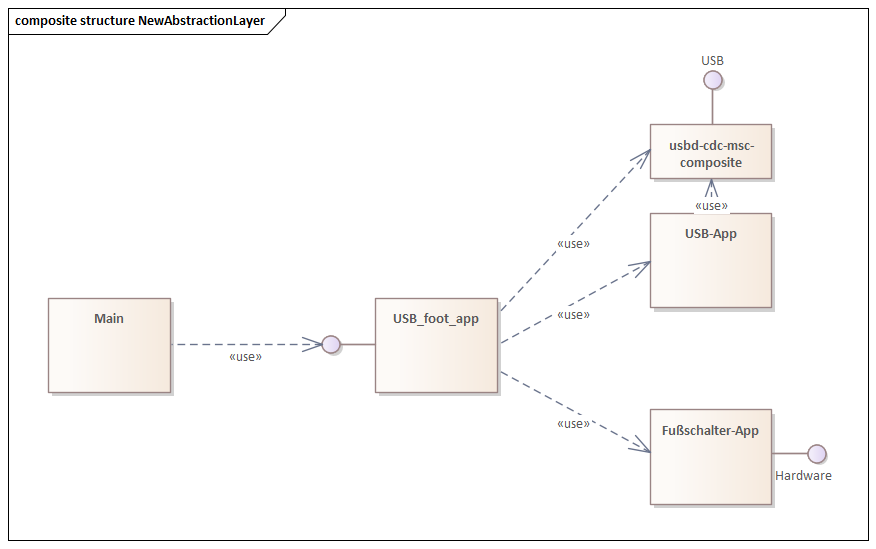
\includegraphics[width=\textwidth]{figures/NewAbstractionLayer.png}
	\caption{Neue Abstraktionsschicht}
\end{figure}

\subsection{USB-HID}
Ein Feature, das sowohl für den Dongle als auch für den Fußschalter implementiert werden soll, ist das Human Interface Device (HID) über USB. In diesem Modus gibt die Anwendung die Messergebnisse nicht mehr über den virtuellen COM-Port aus, sondern ist über USB als Tastatur mit dem Computer verbunden. Über sie werden die Zeichen des Ergebnis als Tastendrücke, gefolgt von einem konfigurierbaren Terminierungszeichen, ausgegeben. Dadurch können Messungen einfach in Excel oder einem Texteditor aufgefangen werde.\\
Für die Implementierung werden die Funktionen des NRF-Library Files app\_usb\_hid\_kbd.h verwendet. Es abstrahiert die Low-Level USB-Aufrufe und stellt Funktionen zur Verfügung, die bei Aufruf eine Taste drücken oder loslassen. Es fehlt jedoch eine Funktion die ganze Strings serialisiert, weshalb diese implementiert werden muss. Die Scancodes, die Nummern der Tasturtasten, sowie der Modifier, eine Taste die Tastendrücke modifiziert, wie die Shift-Taste, werden dabei von einer Funktion erhalten, die im nrf\_Base Projekt enthalten ist. Sie wurde für die HID Implementierung über BLE geschrieben und gibt den Scancode und zugehörigen Modifier für einen ASCII Character zurück.\\
Zwischen den Tastendrücken muss eine gewisse Zeit gewartet werden, da der Computer Tastendrücke zwischen denen zu wenig Zeit verstreicht nicht registriert. Dieser Delay wurde auf 1 Millisekunden festgelegt. Diese Art darauf zu warten, dass die Tastendrücke vom Computer registriert wurde, stellte sich jedoch als sehr fehleranfällig heraus. Nicht nur wurde dopplete Zeichen nicht korrekt erkannt, sondern nach ungefähr 10 Ausgaben schien der USB-Bus überlastet zu sein. Daher musste die Implementierung geändert werden. Statt die Tastendrücken ohne Rücksicht auf die zugehörigen Events dem USB zu übergeben, muss nach jedem Zeichen auf ein Event der USB-HID Library gewartet werden, das die erfolgreiche Übertragung signalisiert. Dazu muss der zu serialisierende String in einem Buffer hinterlegt und bei Empfangen des Events das nächste Zeichen übertragen werden.

\subsection{BLE-HID}
Ein weiterer Modus, in dem der Fußschalter arbeiten soll, ist HID über BLE. Dabei simuliert der Fußschalter oder Dongle eine über BLE verbindbare Tastatur und serialisiert nach dem Verbinden wie bei HID über USB die Messergebnisse als Tastendrücken. Dazu muss das Gerät nun zusätzlich zur Central Rolle in der Peripheral Rolle agieren. Dazu muss einerseits das Advertising korrekt konfiguriert werden und in den bestehenden Code des Peripheren Verbindungsaufbaus, die Fußschalter Applikation eingebunden werden. Für das eigentliche Schreiben des Messergebnisses über BLE, gibt es bereits bestehenden Funktionen des nrf\_Base Projekts die einen String vollständig serialisert und diese muss nur in der Fußschalter Applikation aufgerufen werden. Erste Tests zeigen, dass die Geschwindigkeit der Übertragung, einerseits die Dauer bis angefangen wird das Messergebnis zu schreiben und anderseits wie schnell die einzelnen Tastendrücke erfolgen, zu hoch ist. Bei der Untersuchung wurde dabei bereits ein Bug im nrf\_Base Projekt gefunden.  

\subsection{BLE-Windows-App}
Der letzte Modus, in dem der Fußschalter agieren soll, ist als ein an die HCT-Windows-App angebundenes Gerät. Dabei soll das Signal der Betätigung des Tasters als eine HCT-Nachricht an die Windows-App gesendet werden, welchen dann ein Messergebnis bei den mit ihr verbundenen Messgeräten triggert. Dazu muss ein HCT-Model für den Fußschalter geschaffen werden. Das Model stellt folgende Werte bereit:
\begin{itemize}
	\item Device Class
	\item Protocol type, version 
	\item Version of Hardware, Software, BLE
	\item Battery level, status
	\item Reset 
\end{itemize}

Werte des Config.ini Konfigurationsfiles:
\begin{itemize}
	\item Operating Mode 
	\item CDC protocol 
	\item HID Keyboard Language ID 
	\item HID data set seperator 
	\item HID number seperator
	\item HID single key 
\end{itemize}

Für die Übertragung des eigentlichen Signals, dass der Fußschalter betätigt wurde, muss eine HCT-Charakteristik angelegt werden, auf welche die HCT-Windows-App sich subscriben kann. Über diese Charakteristik wird sie dann über die Betätigung des Tasters notifiziert. Im Advertising muss sich der Fußschalter dann nicht als Tastatur, sondern als HCT-Fußschalter erkenntlich zeigen.